
%(BEGIN_QUESTION)
% Copyright 2014, Tony R. Kuphaldt, released under the Creative Commons Attribution License (v 1.0)
% This means you may do almost anything with this work of mine, so long as you give me proper credit

Calculate the total impedance offered by these two inductors to a sinusoidal signal with a frequency of 60 Hz:

$$\includegraphics[width=15.5cm]{i01031x01.eps}$$

Show your work using two different problem-solving strategies:

\begin{itemize}
\item{} Calculating total inductance ($L_{total}$) first, then total impedance ($Z_{total}$).
\item{} Calculating individual impedances first ($Z_{L1}$ and $Z_{L2}$), then total impedance ($Z_{total}$).
\end{itemize}

Do these two strategies yield the same total impedance value?  Why or why not?

\underbar{file i01031}
%(END_QUESTION)





%(BEGIN_ANSWER)

\noindent
{\bf First strategy:}

$L_{total} = 1.1 \hbox{ H}$

$X_{total} = 414.7 \> \Omega$

${\bf Z_{total}} = 414.7 \> \Omega \> \angle \> 90^o$ or ${\bf Z_{total}} = 0 + j414.7 \> \Omega$

\vskip 10pt

\goodbreak

\noindent
{\bf Second strategy:}

$X_{L1} = 282.7 \> \Omega$ \hskip 10pt ${\bf Z_{L1}} = 282.7 \> \Omega \> \angle \> 90^o$

$X_{L2} = 131.9 \> \Omega$ \hskip 10pt ${\bf Z_{L2}} = 131.9 \> \Omega \> \angle \> 90^o$

${\bf Z_{total}} = 414.7 \> \Omega \> \angle \> 90^o$ or ${\bf Z_{total}} = 0 + j414.7 \> \Omega$

%(END_ANSWER)





%(BEGIN_NOTES)

The purpose of this question is to get students to realize that {\it any} way they can calculate total impedance is correct, whether calculating total inductance and then calculating impedance from that, or by calculating the impedance of each inductor and then combining impedances to find a total impedance.  This should be reassuring, because it means students have a way to check their work when analyzing circuits such as this!

%INDEX% Electronics review: AC reactance and impedance

%(END_NOTES)


